\documentclass[11pt,a4paper]{article}
\usepackage[margin=2.2cm]{geometry}
\usepackage{graphicx,booktabs,amsmath,amssymb,xcolor,float}
\usepackage[colorlinks=true,linkcolor=blue!50!black,urlcolor=blue!50!black]{hyperref}
\usepackage{caption,xurl,microtype}
\captionsetup{font=small}
\newcommand{\pkd}{\textsc{pkdgrav3}}
\newcommand{\gad}{\textsc{Gadget-4}}
\newcommand{\fp}[1]{\nolinkurl{#1}}
\newcommand{\kms}{(km\,s$^{-1}$)$^2$}
\newcommand{\Mpch}{$h^{-1}$\,Mpc}
\newcommand{\Msunh}{$h^{-1}$\,M$_\odot$}

\title{The potential around halos in a finite periodic box,\\ and why potential \emph{differences} are safe}
\author{Sahyadri sandbox, branch \fp{rockstar-pkc-reader}\\
  \small\fp{reports/gadget_pkdgrav3_potential/box_size_note}}
\date{13 November 2026}

\begin{document}
\maketitle

\begin{abstract}
\noindent The volume-weighted stacked potential around halos in the $256^3$, $200$\,\Mpch{} comparison runs of \gad{} and \pkd{} is shallower, and reaches zero at a smaller radius, than the one measured with an independent (HEALPix-based)
code in other simulations. We show that this is what a $200$\,\Mpch{} periodic box must give. The potential is
dominated by long-wavelength modes ($\phi_k\propto\delta_k/k^2$), which a small box does not contain, and a periodic
potential has zero volume mean by construction. In linear theory the profile around a halo in a $200$\,\Mpch{} box is
$21\%$ shallower than in an infinite volume at $1$\,\Mpch, $32\%$ at $15$, $60\%$ at $45$, and crosses zero at
$84$\,\Mpch. The measured stacks of both codes agree with this finite-box prediction within its realisation scatter
at all radii. Boxes of $1$ and $2$\,$h^{-1}$Gpc are within $5\%$ and $1.2\%$ of the infinite-volume profile out to
$45$\,\Mpch. The \emph{difference} of the potential between two halos is almost unaffected: its mean
$\langle\phi_B-\phi_A\rangle$ is changed by $<1\%$ out to $30$\,\Mpch{} even at $L=200$\,\Mpch, because a mode much
longer than the separation shifts both halos equally. Its rms is low by $11$--$20\%$ at $L=200$\,\Mpch, but by only
$\le3\%$ at $500$\,\Mpch{} and $\le1.3\%$ at $1$\,$h^{-1}$Gpc. Absolute potentials and their correlations, on the
other hand, depend strongly on the box (and have no infinite-volume limit for $n_s<1$).
\end{abstract}

\tableofcontents

%======================================================================================================
\section{The question and the checks of the measurement}
\label{sec:checks}

The stacked potential profiles of the comparison report (\fp{halo_potential_profile.py}) were compared with profiles
measured, by a different code, in independent simulations. That code counts particles in HEALPix pixels in radial
shells around each halo, takes the mean potential in each pixel, and averages over the pixels. For the same mass bin
the independent profile is deeper and approaches zero at a much larger radius. Before turning to the box size, we
verified the measurement itself:

\begin{enumerate}
\item \textbf{\gad's potential conventions, from the source} (\fp{gravity/gravity.cc}, \fp{io/snap_io.cc},
  \fp{main/run.cc}). With \fp{EVALPOTENTIAL}, \fp{PMGRID} and \fp{PERIODIC}:
  \begin{itemize}
  \item the softened self-interaction $-Gm/\epsilon$ is removed;
  \item the TreePM zero-point term $\pi G M_{\rm tot}/(\alpha^2L^3)$ is added, so that a uniform background has no
    short-range potential;
  \item the PM part has no $k=0$ mode.
  \end{itemize}
  The written potential therefore has zero \emph{volume} mean. The output is the comoving potential, and the peculiar
  potential is that divided by $a$. The snapshot is written right after a full force evaluation at the output time.
\item \textbf{Amplitude against an independent Poisson solve.} We solved
  $\nabla^2\phi = \tfrac32\Omega_m H_0^2\delta/a$ on a $512^3$ CIC grid, deconvolved for assignment and
  interpolation (\fp{compare_potential.py}). \gad's particle potential has slope $1.007$ against it at $z=0$ and
  $1.001$ at $z=0.5$.
\item \textbf{The stacking code on synthetic data with a known potential.} We used a Gadget-format file with $80^3$
  random particles in a periodic box and $\phi = \sum_h -3\times10^5/(r_h+0.3) + {\rm const}$, stored as $\phi a$.
  \begin{itemize}
  \item The particle-weighted stack equals a brute-force average over (halo, particle) pairs to $10^{-8}$.
  \item The volume-weighted stack equals the exact shell average of $\phi$ to $10^{-3}$ beyond three grid cells. It
    is too shallow inside two cells, because the grid smooths the cusp.
  \end{itemize}
\end{enumerate}

The particle-weighted stack levels off at large $r$ at the mean potential of all particles ($-5.45\times10^5$\,\kms{}
at $z=0$), not at zero. Most particles are in halos, so this is a mass-weighted mean. The volume-weighted stack, which
is what the independent code approximates, goes to zero. The rest of this note concerns the volume-weighted profile.

%======================================================================================================
\section{Linear theory in a finite periodic box}
\label{sec:theory}

\paragraph{Power spectrum and potential.}
We use the cosmology of the runs: $\Omega_m=0.31377$, $\Omega_b=0.04930$, $h=0.6736$, $n_s=0.9649$,
$\sigma_8=0.811$, at $z=0$. The linear matter spectrum is $P(k)=A\,k^{n_s}T^2(k)$, with the no-wiggle transfer
function of Eisenstein \& Hu (1998). $A$ is fixed by $\sigma_8$, the rms of $\delta$ in a top hat of $8$\,\Mpch. BAO
wiggles and the exact transfer function change the ratios below by much less than the effects discussed.

The peculiar potential (physical, \kms{}, comoving $k$ in $h$\,Mpc$^{-1}$, $H_0=100\,h$\,km\,s$^{-1}$Mpc$^{-1}$) is
\begin{equation}
  \phi_{\boldsymbol k} = -\frac{3}{2}\,\frac{\Omega_m H_0^2}{a}\,\frac{\delta_{\boldsymbol k}}{k^2}
  \equiv \mathcal{P}\,\frac{\delta_{\boldsymbol k}}{k^2},
  \qquad \mathcal{P} = -1.5\,\Omega_m\,(100)^2\ \text{at } a=1 .
\end{equation}

\paragraph{Potential profile around halos.}
Halos are linear tracers, $\delta_h=b\,\delta$ on large scales. The volume-weighted mean potential at distance $r$
from a halo, i.e.\ the halo--potential cross-correlation, is then $b\,\xi_{\phi m}(r)$ with
\begin{equation}
  \xi_{\phi m}(r) = \langle \phi(\boldsymbol x+\boldsymbol r)\,\delta(\boldsymbol x)\rangle
  = \mathcal{P}\int\!\frac{d^3k}{(2\pi)^3}\,\frac{P(k)}{k^2}\,j_0(kr)
  = \frac{\mathcal{P}}{2\pi^2}\int_0^\infty\! dk\,P(k)\,j_0(kr),
  \label{eq:prof}
\end{equation}
where $j_0(x)=\sin x/x$ is the spherical average of $e^{i\boldsymbol k\cdot\boldsymbol r}$. Two features matter
here.
\begin{itemize}
\item The weight of a mode is $P(k)\,dk$, not $k^2P(k)\,dk$ as for $\xi_{mm}$. Modes near and below the peak of
  $P(k)$ ($k\approx0.02$\,$h$\,Mpc$^{-1}$, wavelength $\approx300$\,\Mpch) therefore carry much of the profile.
\item The profile decays only slowly: it is still $-0.67\times10^5$\,\kms{} per unit bias at $100$\,\Mpch{}
  (Table~\ref{tab:ratio}).
\end{itemize}

\paragraph{Finite periodic box.}
A periodic box of side $L$ contains only the lattice modes $\boldsymbol k = k_f\boldsymbol n$, with
$k_f=2\pi/L$ and $\boldsymbol n\in\mathbb Z^3$. The mode $\boldsymbol n=0$ is absent: the box mean of $\delta$ is
zero by definition, and that of $\phi$ by the Poisson solver's convention (Sec.~\ref{sec:checks}). The integral
becomes a sum,
\begin{equation}
  \int\!\frac{d^3k}{(2\pi)^3} f(k) \;\longrightarrow\; \frac{1}{L^3}\sum_{\boldsymbol n\ne0} f(k_f|\boldsymbol n|).
  \label{eq:lattice}
\end{equation}

\paragraph{Numerics.}
We evaluate the sum exactly over all lattice points with $|\boldsymbol n|\le n_{\max}$, grouping points by $|\boldsymbol n|^2$
with their multiplicities. Here $n_{\max}=\min(60,\,1.5/k_f)$. Above $k_f n_{\max}$ we use the continuous integral,
where the lattice is dense and the two agree to $\ll1\%$. The sum and the integral must not overlap: an early version
included the corners of the cube $|n_i|\le n_{\max}$, double counted the shell $n_{\max}<|\boldsymbol n|\le\sqrt3n_{\max}$,
and gave ratios above one for large boxes. The infinite-volume integrals use $4\times10^5$ log-spaced $k$ from
$10^{-6}$ to $10^2$\,$h$\,Mpc$^{-1}$ with Simpson's rule. All of this is in \fp{make_boxsize_figures.py} and runs
in 10\,s.

\paragraph{Realisation scatter.}
A single box of side $L$ has only a few modes on the scales that set the profile at large $r$, so its measured stack
scatters around the expected value. For Gaussian fields, the variance of the stacked profile estimator over
realisations is
\begin{equation}
  \sigma^2_{\rm real}(r) = \frac{1}{L^3}\;\frac{1}{L^3}\sum_{\boldsymbol n\ne0}
  \Big[P_{\phi\phi}(k)\big(b^2P(k)+\bar n_h^{-1}\big) + \big(b\,P_{\phi m}(k)\big)^2\Big]\,j_0^2(kr),
  \label{eq:cv}
\end{equation}
with $P_{\phi m}=\mathcal{P}P/k^2$, $P_{\phi\phi}=\mathcal{P}^2P/k^4$, and $\bar n_h$ the number density of the
stacked halos. The two terms are the Gaussian (disconnected) covariance of the estimator
$\hat\xi_{\phi h}(r)\propto\sum_{\boldsymbol k}\phi_{\boldsymbol k}\delta^*_{h,\boldsymbol k}\,j_0(kr)$. We
neglect the shot noise of the particles that carry $\phi$ ($\bar n = 2.1$ particles per (\Mpch)$^3$, a negligible
term on these scales). This is the band in Fig.~\ref{fig:meas}. The jackknife errors of the stacks measure only the scatter
within the one box, not this.

\paragraph{Halo bias.}
To compare with the measurement without free parameters, we take $b$ for each mass bin from the same run. It is the
least-squares ratio of the measured halo--matter cross-correlation (the particle-count excess $\delta_{hm}$ of the
particle-weighted stack) to the linear $\xi_{mm}$ of the $200$\,\Mpch{} box, over $20<r<40$\,\Mpch. This gives
$b=0.70,\,0.98,\,1.53,\,2.28$ (\gad) and $0.67,\,0.99,\,1.57,\,2.23$ (\pkd) for $M_{\rm vir}$ in
$[2\times10^{12},10^{13})$, $[10^{13},5\times10^{13})$, $[5\times10^{13},2\times10^{14})$ and $\ge2\times10^{14}$\,\Msunh.

%======================================================================================================
\section{Results: the profile around halos}
\label{sec:profile}

\begin{figure}[t]
\centering
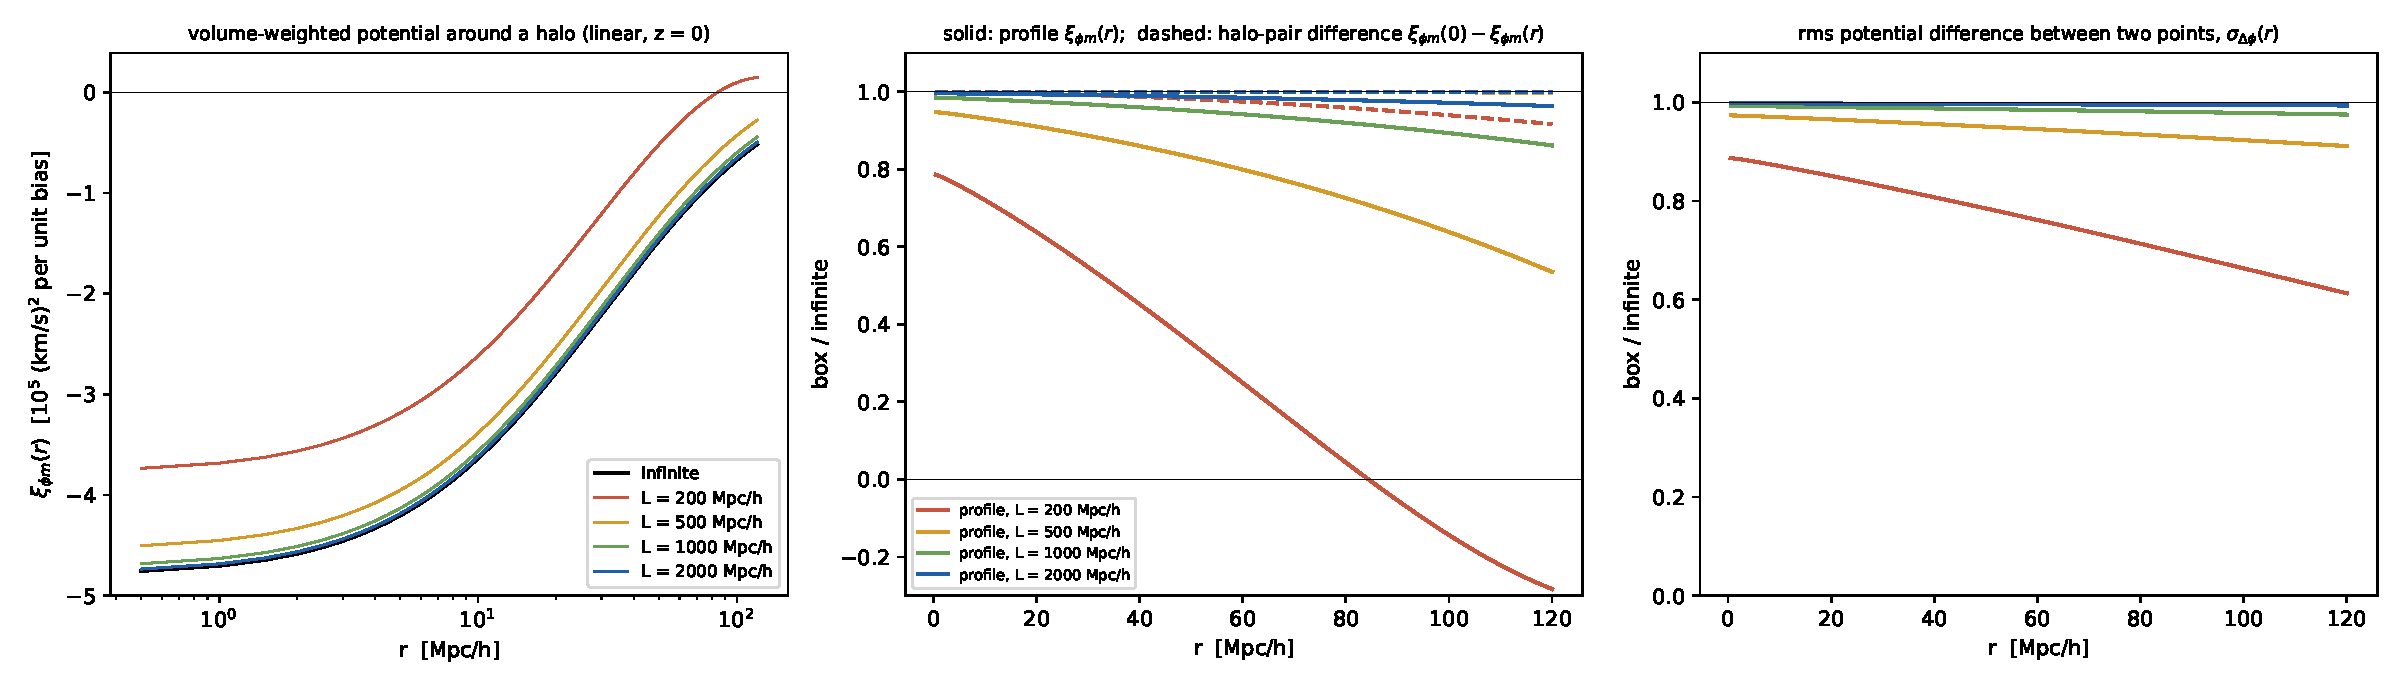
\includegraphics[width=\textwidth]{figs/boxsize_theory.pdf}
\caption{Linear theory at $z=0$. \emph{Left:} the volume-weighted potential around a halo per unit bias,
Eq.~\eqref{eq:prof}, for an infinite volume and for periodic boxes. \emph{Middle:} box over infinite volume for the
profile (solid) and for the mean potential difference between two halos, Eq.~\eqref{eq:pair} (dashed; the curves for
$L\ge500$\,\Mpch{} lie on top of one another at 1). \emph{Right:} the same for the rms potential difference between
two points, Eq.~\eqref{eq:sf}.}
\label{fig:theory}
\end{figure}

\begin{table}[H]
\centering\small
\caption{Volume-weighted potential around a halo, per unit bias, in linear theory at $z=0$: the infinite-volume
value ($10^5$\,\kms) and the ratio box/infinite.}
\label{tab:ratio}
\begin{tabular}{@{}lrrrrrrrrr@{}}
\toprule
$r$ [\Mpch] & 1 & 5 & 10 & 15 & 20 & 30 & 45 & 70 & 100 \\
\midrule
$\xi_{\phi m}$, infinite [$10^5$\,\kms] & $-4.70$ & $-4.20$ & $-3.64$ & $-3.17$ & $-2.79$ & $-2.20$ & $-1.62$ & $-1.05$ & $-0.67$\\
$L=200$\,\Mpch  & 0.78 & 0.76 & 0.72 & 0.68 & 0.64 & 0.55 & 0.40 & 0.15 & $-0.14$ \\
$L=500$         & 0.95 & 0.94 & 0.93 & 0.92 & 0.91 & 0.89 & 0.85 & 0.76 & 0.64 \\
$L=1000$        & 0.99 & 0.98 & 0.98 & 0.98 & 0.97 & 0.97 & 0.96 & 0.93 & 0.89 \\
$L=2000$        & 1.00 & 1.00 & 1.00 & 0.99 & 0.99 & 0.99 & 0.99 & 0.98 & 0.97 \\
\bottomrule
\end{tabular}
\end{table}

A small box makes the profile both shallower and shorter in range (Fig.~\ref{fig:theory}, Table~\ref{tab:ratio}).
\begin{itemize}
\item \textbf{Depth.} Even at the halo centre a $200$\,\Mpch{} box is $\sim20\%$ shallower, because the missing long
  modes set the potential level of a whole region.
\item \textbf{Range.} The deficit grows with $r$. At $L=200$\,\Mpch{} the profile crosses zero at $84$\,\Mpch{} and is
  positive beyond, as required by the zero volume mean: the potential deficit around a halo must be balanced
  elsewhere in the box. In an infinite volume it is still $-0.67\times10^5$\,\kms{} per unit bias at $100$\,\Mpch.
\end{itemize}
These are the two differences seen between our profiles and the independent ones. By $L=1\,h^{-1}$Gpc the profile is
within $5\%$ of the infinite-volume one out to $45$\,\Mpch; at $2\,h^{-1}$Gpc, within $1.2\%$.

\begin{figure}[t]
\centering
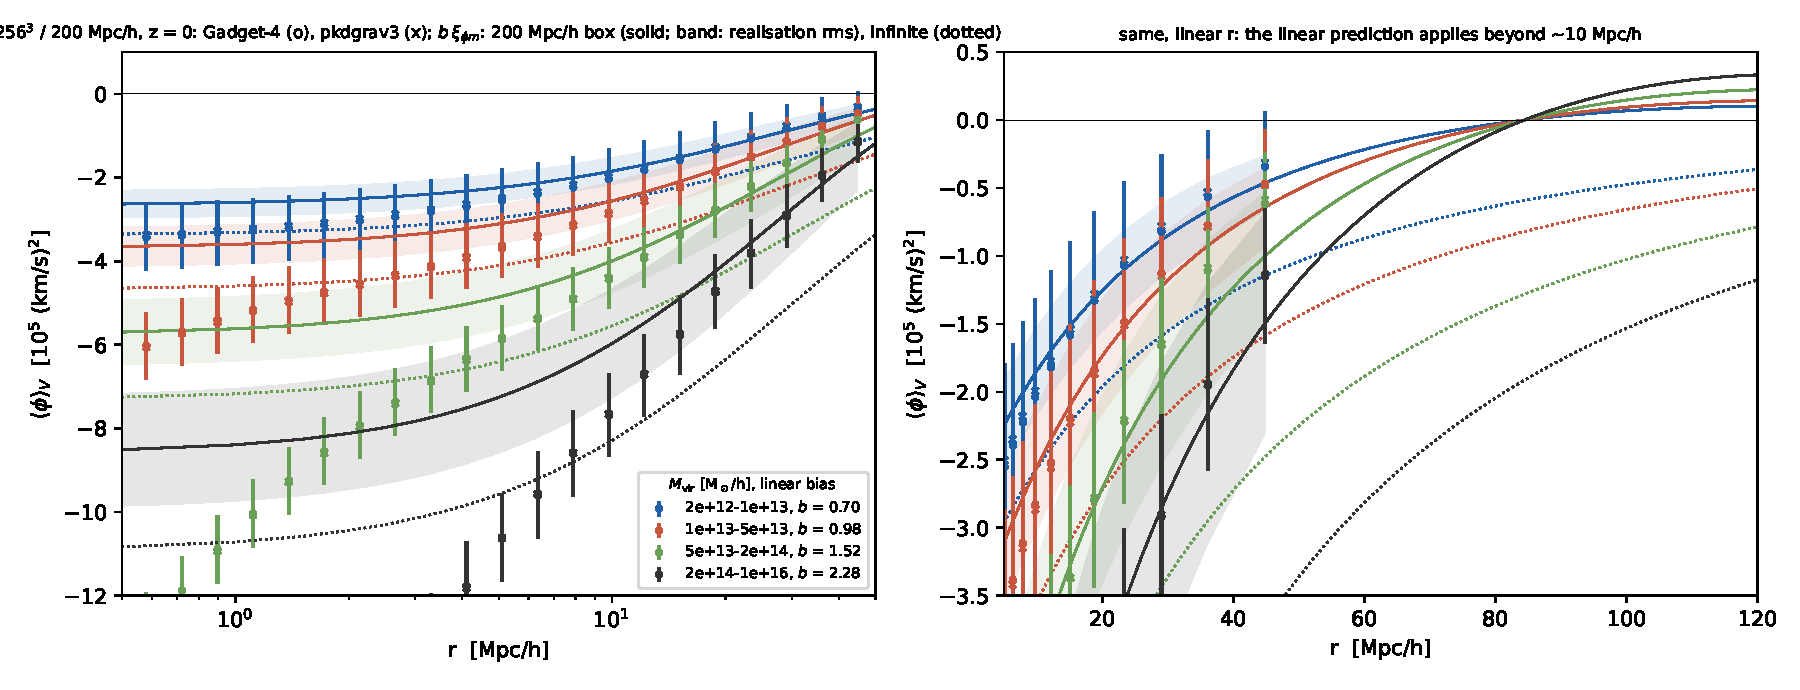
\includegraphics[width=\textwidth]{figs/boxsize_measured.pdf}
\caption{Measured volume-weighted stacks of the $256^3$, $200$\,\Mpch{} runs at $z=0$: \gad{} (circles, jackknife
errors) and \pkd{} (crosses), for four mass bins. Curves: $b\,\xi_{\phi m}$ in the $200$\,\Mpch{} box (solid; band:
realisation rms, Eq.~\eqref{eq:cv}) and in an infinite volume (dotted), with $b$ measured from the halo--matter
cross-correlation. \emph{Left}: log $r$; \emph{right}: linear $r$, with the predictions continued to $120$\,\Mpch.
Linear theory does not describe the inner few \Mpch{}, which are dominated by the halo's own potential well.}
\label{fig:meas}
\end{figure}

\paragraph{Comparison with the measured stacks.}
The measured stacks of both codes follow the $200$\,\Mpch{} prediction, not the infinite-volume one
(Fig.~\ref{fig:meas}).
\begin{itemize}
\item Between $12$ and $45$\,\Mpch{} the ratio measured/predicted runs from $1.07$ to $0.74$ for the lowest mass bin
  (similar for the others).
\item The realisation scatter of the prediction, Eq.~\eqref{eq:cv}, is $19\%$ of the signal at $12$\,\Mpch{} and
  $44\%$ at $45$\,\Mpch, so the deviations are $-0.4$ to $+0.8\,\sigma_{\rm real}$ for the three lower mass bins and
  $-1.0$ to $+0.5\,\sigma_{\rm real}$ for the highest.
\item The infinite-volume curve is excluded at large $r$. At $45$\,\Mpch{} it is about three times as deep as the
  measurement.
\end{itemize}
\pkd{} and \gad{} agree to $1$--$3\%$ inside $15$\,\Mpch{} and to $3\times10^3$\,\kms{} ($<0.1$ jackknife
$\sigma$) at $45$\,\Mpch, as they must: the same initial conditions have the same missing modes.

\paragraph{The estimator.}
The independent HEALPix estimator differs from ours in two ways, each of which makes it deeper:
\begin{itemize}
\item Within a pixel it averages \emph{particles}, so the dense (deeper) part of the pixel counts more.
\item Empty pixels, which lie preferentially in underdense regions with high $\phi$, drop out of the average.
\end{itemize}
Both are largest at small $r$ and where few particles fall in a pixel. At large $r$, where pixels are big and well
filled, the pixel mean approaches a mass-weighted mean. That tends to the particle-mean level rather than to zero, and
so also delays the approach to zero. The size of this effect can be measured directly by running the HEALPix estimator
on the same snapshots; it is independent of the box-size effect above.

%======================================================================================================
\section{Does this matter for potential differences between halos?}
\label{sec:diff}

Observables such as gravitational redshifts compare the potential at two places, and the halo cross-correlation tools
of this branch use per-halo potentials. We therefore distinguish three quantities.

\paragraph{1. Mean potential difference between two halos.}
Take halos of bias $b_A$ and $b_B$ at separation $r$. To linear order in Gaussian fields,
$\langle\phi(\boldsymbol x_B)\,|\,{\rm halos\ at\ }\boldsymbol x_A,\boldsymbol x_B\rangle = b_A\,\xi_{\phi m}(r) + b_B\,\xi_{\phi m}(0)$:
halo $B$ sits in its own potential well and in the outskirts of $A$'s. Hence
\begin{equation}
  \langle\phi_B-\phi_A\rangle(r) = (b_B-b_A)\,\big[\xi_{\phi m}(0)-\xi_{\phi m}(r)\big]
  = (b_B-b_A)\,\frac{\mathcal{P}}{2\pi^2}\int\! dk\,P(k)\,\big[1-j_0(kr)\big].
  \label{eq:pair}
\end{equation}
A mode with $kr\ll1$ contributes $\propto(kr)^2/6$: it raises or lowers both halos by the same amount and cancels in
the difference. The box therefore removes almost nothing.

\begin{table}[H]
\centering\small
\caption{Mean potential difference between two halos per unit bias difference, Eq.~\eqref{eq:pair}, and the rms
potential difference between two points, Eq.~\eqref{eq:sf}: infinite-volume values and box/infinite.}
\label{tab:diff}
\setlength{\tabcolsep}{4pt}
\begin{tabular}{@{}lrrrrrrrrr@{}}
\toprule
$r$ [\Mpch] & 1 & 5 & 10 & 15 & 20 & 30 & 45 & 70 & 100 \\
\midrule
$\xi_{\phi m}(0)-\xi_{\phi m}(r)$, inf.\ [$10^5$\,\kms] & $-0.08$ & $-0.58$ & $-1.15$ & $-1.62$ & $-2.00$ & $-2.58$ & $-3.17$ & $-3.74$ & $-4.12$\\
\quad $L=200$\,\Mpch & 1.00 & 1.00 & 1.00 & 1.00 & 0.99 & 0.99 & 0.98 & 0.97 & 0.94 \\
\quad $L=500$        & 1.00 & 1.00 & 1.00 & 1.00 & 1.00 & 1.00 & 1.00 & 1.00 & 1.00 \\
\midrule
$\sigma_{\Delta\phi}(r)$, inf.\ [$10^5$\,\kms] & 0.27 & 1.33 & 2.57 & 3.72 & 4.80 & 6.77 & 9.34 & 12.9 & 16.3 \\
\quad $L=200$\,\Mpch & 0.89 & 0.88 & 0.87 & 0.86 & 0.85 & 0.83 & 0.80 & 0.74 & 0.66 \\
\quad $L=500$        & 0.97 & 0.97 & 0.97 & 0.97 & 0.97 & 0.96 & 0.95 & 0.94 & 0.92 \\
\quad $L=1000$       & 0.99 & 0.99 & 0.99 & 0.99 & 0.99 & 0.99 & 0.99 & 0.98 & 0.98 \\
\bottomrule
\end{tabular}
\end{table}

Even in the $200$\,\Mpch{} box, the mean difference is within $1\%$ of the infinite-volume value out to $30$\,\Mpch{}
and within $3\%$ at $70$\,\Mpch{} (Table~\ref{tab:diff}). From $500$\,\Mpch{} on, the difference is exact to the
precision shown. The term $\xi_{\phi m}(0)$ is the linear part of the halo's own potential; its non-linear part
(the halo's internal well) comes from small scales and does not depend on the box at all.

\paragraph{2. Scatter of the potential difference (structure function).}
The rms difference of $\phi$ between two points at separation $r$ is
\begin{equation}
  \sigma^2_{\Delta\phi}(r) = \big\langle[\phi(\boldsymbol x+\boldsymbol r)-\phi(\boldsymbol x)]^2\big\rangle
  = 2\mathcal{P}^2\!\int\!\frac{d^3k}{(2\pi)^3}\,\frac{P(k)}{k^4}\big[1-j_0(kr)\big].
  \label{eq:sf}
\end{equation}
At small $k$ the integrand goes as $P(k)\,r^2$, which converges but gives weight to wavelengths around and above
$r$. A $200$\,\Mpch{} box is $11$--$20\%$ low between $1$ and $45$\,\Mpch, $500$\,\Mpch{} is $3$--$5\%$ low, and
$1\,h^{-1}$Gpc is $1\%$ low. This is the large-scale (two-halo) part of the structure function \fp{sf} of
\fp{halo_potential_xcorr.py}. The halo-to-halo scatter of the potential wells adds to it independently of the box,
which reduces the fractional effect on the measured \fp{sf}.

\paragraph{3. Absolute potentials and their correlation.}
The covariance of the potential at two points,
$\xi_{\phi\phi}(r)=\mathcal{P}^2\int\! d^3k/(2\pi)^3\,P(k)k^{-4}j_0(kr)$, has an integrand $\propto k^{n_s-2}$ at
small $k$. For $n_s<1$ it diverges in an infinite volume, so the absolute potential has no infinite-volume rms. In a
box, both the rms and the correlation keep growing with $L$:

\begin{table}[H]
\centering\small
\begin{tabular}{@{}lrrrrr@{}}
\toprule
$L$ [\Mpch] & 200 & 500 & 1000 & 2000 & 8000\\
\midrule
rms of $\phi$ (linear) [$10^5$\,\kms] & 7.5 & 14.8 & 20.6 & 26.0 & 35.2 \\
correlation coefficient of $\phi$ at $r=45$\,\Mpch & 0.50 & 0.82 & 0.90 & 0.94 & 0.96 \\
\bottomrule
\end{tabular}
\end{table}

The modes between $2\pi/2000$ and $2\pi/200$\,$h$\,Mpc$^{-1}$, present in a $2\,h^{-1}$Gpc box but not in ours, add
to the potential of every halo a smooth random field with rms $2.3\times10^6$\,\kms. That is larger than the depth of
the halos' own wells. It is coherent over hundreds of \Mpch, so it drops out of differences between neighbouring
halos (points 1 and 2) but not out of absolute values.

\paragraph{Consequences for this branch.}
\begin{itemize}
\item \textbf{Code comparison (\gad{} vs \pkd).} Unaffected: both runs have the same initial conditions and therefore
  the same set of modes.
\item \textbf{Absolute stacked profiles.} These need large boxes. At $L\ge1\,h^{-1}$Gpc the profile is within $5\%$ of
  the infinite-volume one to $45$\,\Mpch{}. The $200$\,\Mpch{} profiles should not be compared in absolute terms with
  those of larger boxes.
\item \textbf{\fp{halo_potential_xcorr.py}.}
  \begin{itemize}
  \item \fp{mean_diff} $=\langle\phi_i-\phi_j\rangle$ is robust (point 1).
  \item \fp{sf} has a box dependence of $\sim15\%$ at $200$\,\Mpch{} and $\lesssim3\%$ from $500$\,\Mpch{} on
    (point 2).
  \item \fp{cov} and \fp{corr} of the absolute potentials are dominated by the longest modes of the box and are not
    comparable between box sizes (point 3).
  \end{itemize}
\item \textbf{Gravitational-redshift dipole of \fp{halo_xi_multipoles.py}.} Each halo is shifted by
  $-\phi/(c\,aH)$. A long mode moves a pair of neighbouring halos together and does not change their separation. The
  long-mode field of rms $2.3\times10^6$\,\kms{} is a coherent shift of $0.08$\,\Mpch. The odd multipoles respond to
  the relative shift $\propto\phi_B-\phi_A$, whose mean is box-independent (point 1). The dipole is therefore
  insensitive to the box size, apart from the usual sample variance of a small volume.
\end{itemize}

%======================================================================================================
\section{Reproducing}

\begin{verbatim}
cd reports/gadget_pkdgrav3_potential/box_size_note
python3 make_boxsize_figures.py   # figs/*.pdf, numbers.json (10 s)
latexmk -pdf boxsize_note.tex
\end{verbatim}
The script reads the reduced $z=0$ stacks in \fp{../data/pkd256_vs_gadget256_r1/profiles/}
(\fp{\{gadget,pkd\}_out100\{,_vol\}.npz}). All numbers quoted here are in \fp{numbers.json}.

\end{document}
